%--------------------
% Packages
% -------------------
\documentclass[12pt,a4paper]{article}
\usepackage[utf8x]{inputenc}
\usepackage[T1]{fontenc}
\usepackage{mathptmx} % Use Times Font


\usepackage[pdftex]{graphicx} % Required for including pictures
\usepackage[czech]{babel} % Swedish translations
\usepackage[pdftex,linkcolor=black,pdfborder={0 0 0}]{hyperref} % Format links for pdf
\usepackage{calc} % To reset the counter in the document after title page
\usepackage{enumitem} % Includes lists

\frenchspacing % No double spacing between sentences
\linespread{1.2} % Set linespace
\usepackage[a4paper, lmargin=0.1666\paperwidth, rmargin=0.1666\paperwidth, tmargin=0.1111\paperheight, bmargin=0.1111\paperheight]{geometry} %margins
%\usepackage{parskip}

\usepackage[all]{nowidow} % Tries to remove widows
\usepackage[protrusion=true,expansion=true]{microtype} % Improves typography, load after fontpackage is selected
\usepackage{xcolor}

\usepackage{lipsum} % Used for inserting dummy 'Lorem ipsum' text into the template
\usepackage{lscape}
\usepackage{subcaption}

%-----------------------
% Set pdf information and add title, fill in the fields
%-----------------------
\hypersetup{ 	
pdfsubject = {IPK},
pdftitle = {Sniffer},
pdfauthor = {Pavel Yadlouski}
}

\begin{document} %All text i dokumentet hamnar mellan dessa taggar, allt ovanför är formatering av dokumentet

\begin{titlepage}
   \begin{center}
        \vspace*{1cm}
        \begin{figure}[h!]
            \centering
            
\includegraphics[width=\textwidth,height=\textheight,keepaspectratio]
            {VUT-FIT-logo-en.png}
        \end{figure}    

        \vspace{0.8cm}
        \large{

        \textbf{Project IDS\\Gallery}

        \vspace{0.5cm}
            Database
        \vspace{1.5cm}

        \textbf{Pavel Yadlouski (xyadlo00)\\Oleksii Korniienko (xkorni02)}

        \vfill
                

        Brno University of Technologies\\
        April, 2020
        }
   \end{center}
\end{titlepage}

\section{Task}

Navrhněte IS pro galerii. Galerii tvoří několik místností (každá místnost 
obsahuje konkrétní expoziční místa různého typu - např. zeď, podlaha), ve kterých
si umělci nebo agentury mohou pronajímat jednotlivá místa pro expozice svých 
uměleckých děl. Pronajímaná místa se liší co do velikosti, ceny, typu a 
dostupného vybavení (např. podstavec, osvětlení, bezpečnostní prvky, atd.). 
Systém by měl evidovat kdo si dané místo pronajal, od kdy do kdy a pro jakou 
expozici. Za každé místo zodpovídá příslušný zaměstnanec galerie. Systém by měl 
také uchovávat informace o expozicích jednotlivých umělců. Tyto informace by měly 
zahrnovat časový rozsah a typ expozice, konkrétní umělecká díla, jejich 
umístění atd. Dále systém musí umožňovat jednoduché vyhledávání umělců, jejich 
děl (podle typu, umístění, klíčového slova, atd.) a poskytovat souhrnné 
statistiky o umělcích, agenturách, expozicích, apod.). Umělci či agentury, 
které hodlají vystavovat, musí do sjednaného data uhradit příslušné poplatky, 
přičemž systém by měl poskytovat hlavnímu provozovateli (jen jemu) informace o 
všech poplatcích (zaplacených i nezaplacených).

\newpage
\section{ER diagram}

Here is entity relationship diagram
\begin{figure}[h!]
    \centering
    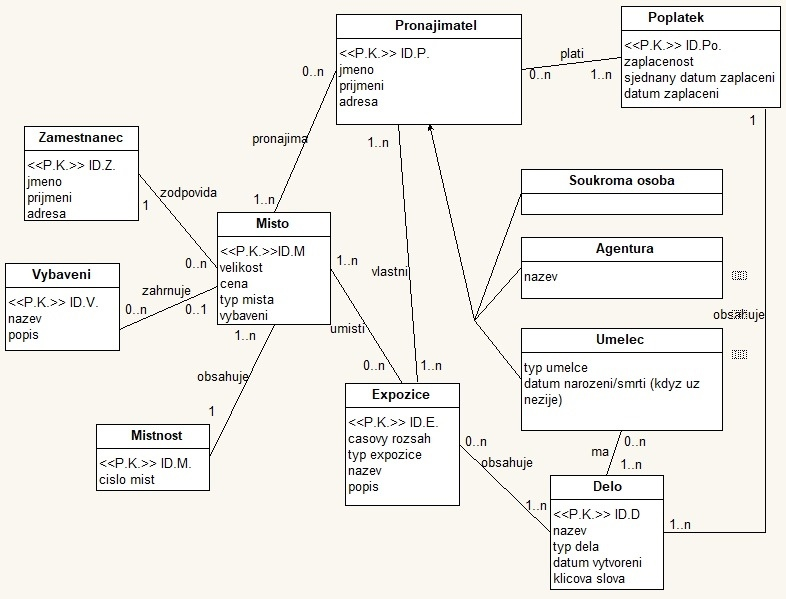
\includegraphics[width=\textwidth,height=\textheight,keepaspectratio]{ER.jpg}
\end{figure}

\newpage
\subsection{Transformed diagram}

For implementation of database we transformed entity relationship diagram to 
database diagram

\begin{figure}[h!]
    \centering
    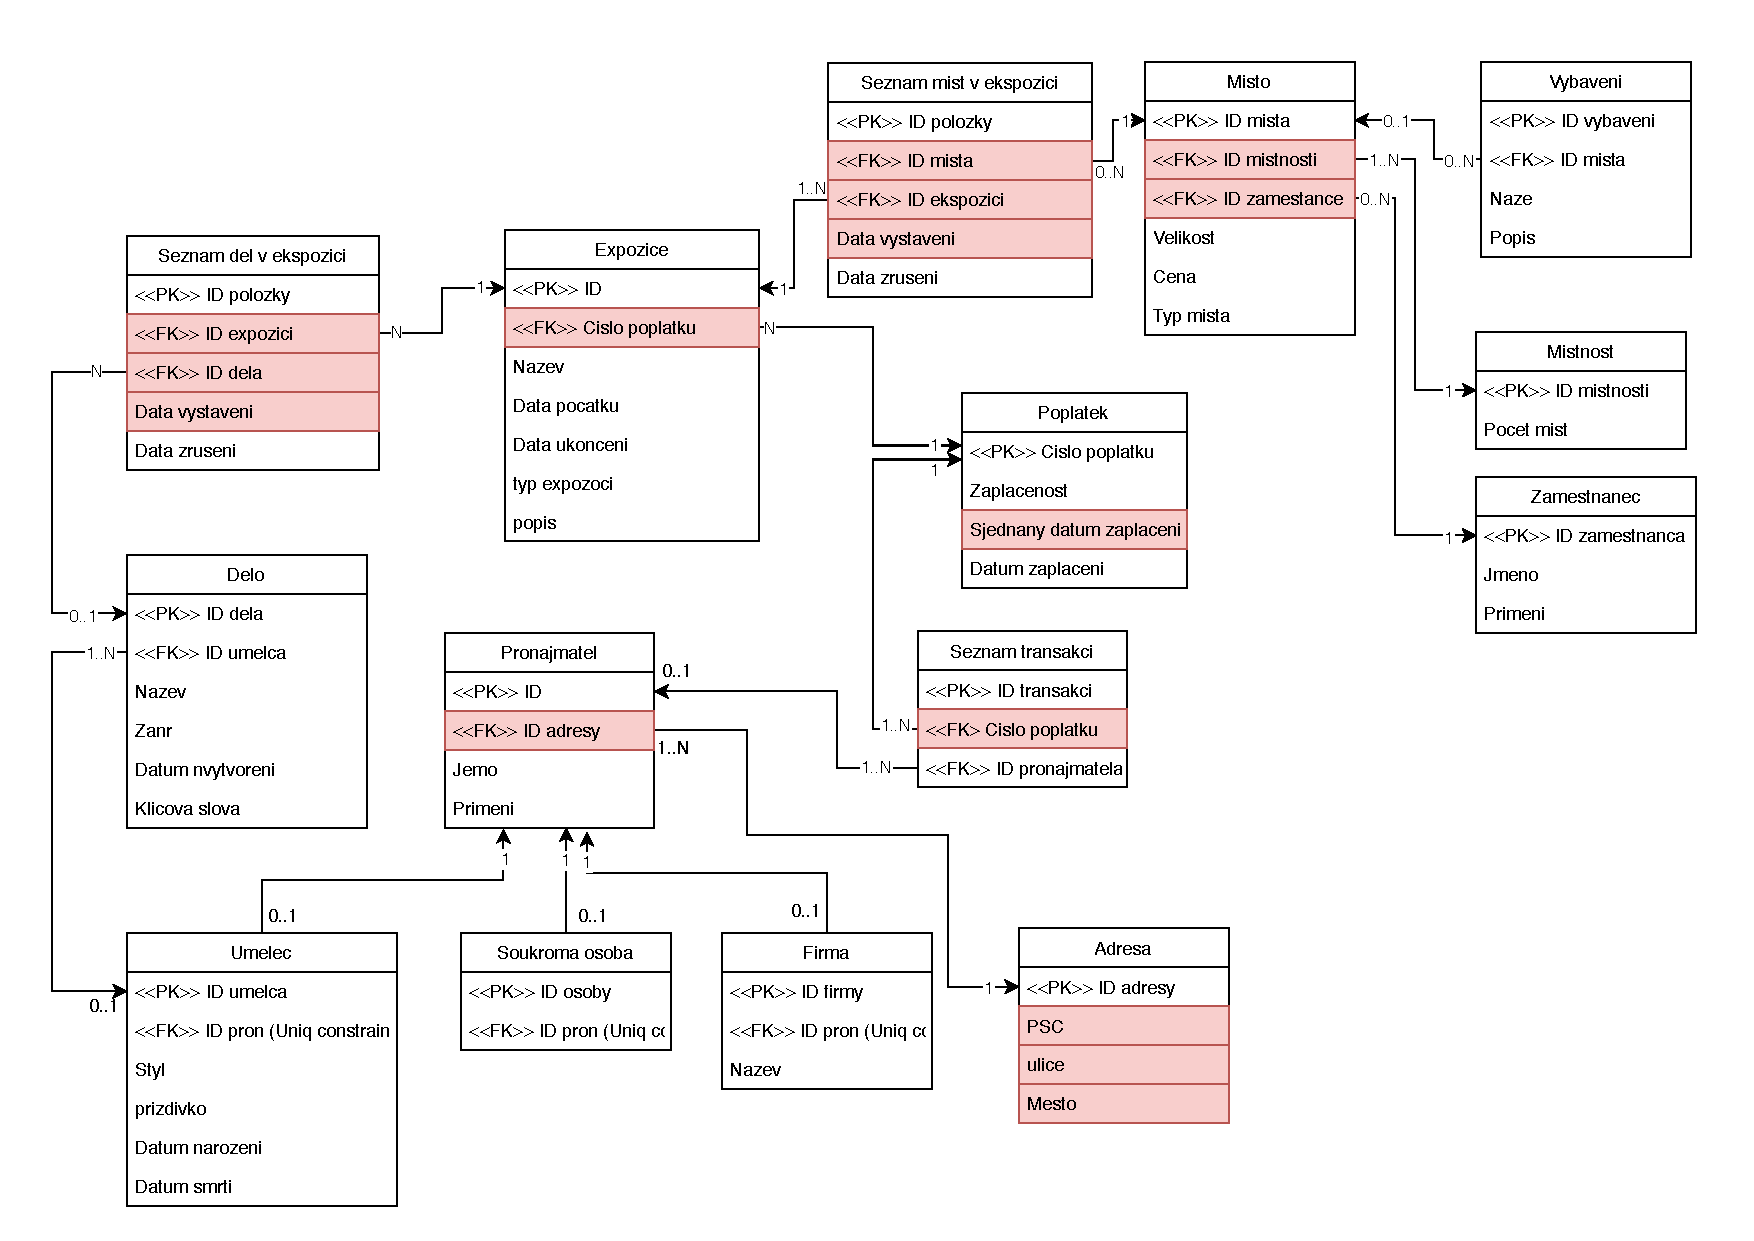
\includegraphics[width=\textwidth,height=\textheight,keepaspectratio]
    {db_diagram.pdf}
\end{figure}

\section{Implementation}

\subsection{Triggers}

There are two triggers: \textit{CHANGE\_NULL\_IN\_VYBAVENI} and 
\textit{SEQ\_VYBAVENI}

\subsubsection{CHANGE\_NULL\_IN\_VYBAVENI}

This trigger is used for changing row \textit{popis} in tabel \textit{EXPOZICE} 
if there is NULL value to sting 'neni popis'. This trigger works on insert to 
given tabel. In first implementation there was problem with muting tables and 
trigger couldn't work. This problem is solved using compound DML triggers.
\begin{figure}[h!]
    \centering
        \includegraphics[width=\textwidth,height=\textheight,keepaspectratio]{before_triger_popis.png}
        \caption{Before using trigger}
        
        \includegraphics[width=\textwidth,height=\textheight,keepaspectratio]{after_triger_popis.png}
        \caption{With using trigger}
\end{figure}

\newpage
\subsubsection{SEQ\_VYBAVENI}

This trigger represents auto increment. Without trigger when there is NULL value 
in ID colum, then there would be an error
\begin{figure}[h!]
    \centering
    \includegraphics[width=\textwidth,height=\textheight,keepaspectratio]{before_trigger_seq.png}
    \caption{Before using auto increment trigger}
\end{figure}

\noindent With using trigger, NULL value in column ID would be replaced with next value 
of sequence
\begin{figure}[h!]
    \centering
    \includegraphics[width=\textwidth,height=\textheight,keepaspectratio]{after_triger_seq.png}
\end{figure}

\newpage

\subsection{Procedures}
Also, there are two procedures: \textit{CHANGE\_POPIS} and \textit{COST\_CHECK}.

\subsubsection{CHANGE\_POPIS}

This procedure is designed to adjust the ABC table so that the item description 
is not blank. The description changes as follows: if there is at least one 
object that is not placed anywhere, then the description of the objects (which 
did not exist before) will be "used" or "not used", otherwise the description 
will be "description not specified".

\begin{figure}[h!]
    \centering
    \includegraphics[width=\textwidth, height=\textheight, keepaspectratio]{before_chahge_popis.jpg}
    \caption{Before using procedure}

    \includegraphics[width=\textwidth, height=\textheight, keepaspectratio]
    {after_change_popis.jpg}
    \caption{After using procedure}
\end{figure}
\newpage
\subsubsection{COST\_CHECK}

This procedure is designed to calculate the cost of one square meter of each 
place separately. If the area is not yet calculated (0) will issue a warning, 
otherwise it will calculate and display a table of results.
\begin{figure}[h!]
    \centering
    \includegraphics[scale=0.6]
    {procedure_check.jpg}
    \caption{Running procedure \texttt{COST\_CHECK}}
\end{figure}

\subsection{Explain plan}

Query is used for selecting column same rows from table \textit{mista} with value 
in column \textit{typ\_mista} equals to \textit{stena}

\begin{figure}[h!]
    \centering
    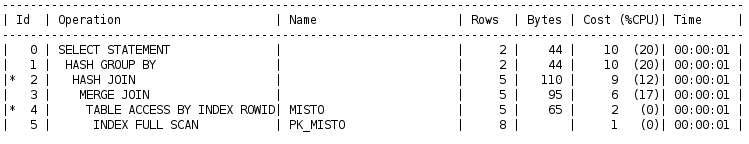
\includegraphics[width=\textwidth,height=\textheight,keepaspectratio]
    {prev_explain_plan.png}
\end{figure}

\noindent After using indexing on column \textit{typ\_mista}

\begin{figure}[h!]
    \centering
    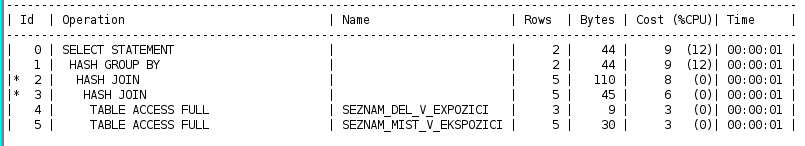
\includegraphics[width=\textwidth,height=\textheight,keepaspectratio]
    {new_explain_plan.png}
\end{figure}

\noindent you can see improvement in CPU usage

\subsection{Materialized view}

The materialized view is used to collect and save the result of a table 
requirement without overflowing. In our case, the view (\textit{MY\_VIEW}) is 
created for another user's table (xkorni02), pre-granting privileges using 
\textit{GRANT} for xyadlo00. The look should reflect the values of each place 
type in all areas.

\end{document}